% !TEX root = ba_doc.tex
\begin{markdown}
\section{Implementation} \label{implementation}

## Architecture

The architecture for ZHAWo consists of a frontend React web application \cite{React} and a backend REST server. The server is implemented with the Node.js \cite{Node} framework Express \cite{Express}. The frontend fetches data such as timetables, mensa menus and event feeds from the backend through a REST API. The backend server - apart from providing the REST API for the frontend - fetches timetable and menu data from the CampusInfo REST API provided by the ZHAW and fetches vszhaw news and calendar events through their RSS feed \cite{VszhawNews} and their calendar application \cite{VszhawCalendar}.

\bigskip
\bigskip

\begin{figure}[H]
  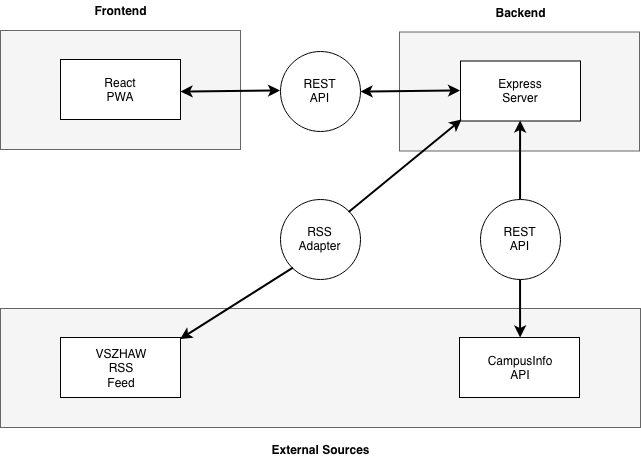
\includegraphics[width=14cm, center]{../../diagrams/applicationArchitecture.png}
  \captionsetup{width=13.5cm}
  \caption[Application architecture diagram]{\textbf{Application architecture diagram}: React frontend application communicating with backend Express server through a REST API. Express server fetches data from vszhaw RSS feed and calendar web application as well as the CampusInfo REST API for timetable and menu data.}
\end{figure}

\newpage

## Backend

The backend architecture consists of the following modules:

\begin{itemize}
  \item \textbf{Express server application}: Handles HTTP requests from frontend and redirection to persistance layer or third-party adapters.
  \item \textbf{Persistence layer}: Handles caching of more resource intensive requests such as room search. Implemented with basic file system using JSON file in the prototype. Can be extended by database if functionality requires.
  \item \textbf{REST API adapter}: Handles HTTP fetch requests to the CampusInfo API.
  \item \textbf{Vszhaw adapter}: Handles fetching of RSS feed and calendar events from vszhaw.
\end{itemize}

### Express Server Application

For the backend server application, we have chosen to use the framework Express \cite{Express} based on the Node.js \cite{Node} technology. The server offers a REST API to get all the data the frontend needs. Most of the server logic handles redirecting user requests from the frontend to either the persistence layer or the different API adapters and then serve the data. Express is the most used JavaScript web application framework with these capabilities. We chose to implement the backend with a JavaScript based framework so there is no technology difference between front- and backend. In the context of agile development in a small team, this allows for a fast implementation of features. A new feature often requires changes to both front- and backend, and by removing the need to switch context between different programming languages, we were able to maintain a good velocity throughout our sprints.

### Persistence Layer

In the scope of this project, there was no need to implement a full database for data persistence. The data for more resource intensive requests such as the search for free rooms is currently stored in JSON format directly in the servers file system. Less intensive requests such as timetables are delivered from CampusInfo in a format that only needs minimal modifications and are directly sent to the frontend without persistence.

However, should the need for a database later arise through new functionality, integration into the Express server application is already prepared.

### REST API Adapter

Most of the application data for ZHAWo is provided by the CampusInfo API. Since this is a third-party API provided by the ZHAW, we decided to implement an additional layer between our backend application core and the API. This insures that we are flexible to changes to CampusInfo.

### Vszhaw adapter

Similarly to the CampusInfo API adapter, the vszhaw adapter provides an additional layer between our application and the RSS feed \cite{VszhawNews} of the vszhaw as well as the calendar web application \cite{VszhawCalendar}. This ensures that should the data received by this third-party feed and calendar application change, that changes needed to our application will be isolated to the adapter.

## Frontend

The frontend is made up of three main parts:

\begin{itemize}
  \item \textbf{React web application}: Handles presentation of data and user interaction.
  \item \textbf{REST API adapter}: Handles HTTP fetch requests to the backend.
  \item \textbf{Service worker}: Handles PWA functionality such as caching of data for offline use and installation to desktop or phone homescreen.
\end{itemize}

### React Web Application

For the presentation of the web application to the user, we used the React framework \cite{React}. React was originaly developed by Facebook and is one of the most popular UI libraries in web development. It is based on reusable components built with JSX, a syntax extension to JavaScript. We decided to use React because of its component based modularity, which works well with an agile development approach where multiple features need to be implemented simultaneously with little interference.

To handle the application data we chose to use the Flux design pattern \cite{Flux}. Using the Flux pattern ensures a unidirectional data flow from view components through actions into a single dispatcher into data stores, where the application data such as timetables and menu plans is handled (Figure \ref{fig:FluxDiag}). In Flux, the dispatcher is a singleton that directs the flow of data to ensure that updates do not cascade, which would lead to unpredictable behavior. When a user interacts with a React view, the view sends an action through the dispatcher, which notifies the stores that hold the application’s data. When the stores change state, the view gets notified and changes accordingly \cite{Flux}.

### REST API Adapter

The data such as timetables, menu plans or lists of free rooms are provided by the backend REST API. To ensure modularity between front- and backend, we implemented an adapter module that handles all data requests to the backend. This practice allows easier adaptations to changes in API, as only the adapter would have to be changed, while the other parts such as the React application and service worker do not need to change.

The modularity this design choice provides - similarly to the modularity of React - goes well with the agile principle of fast prototyping of new ideas and features.

\bigskip

\begin{figure}[H]
  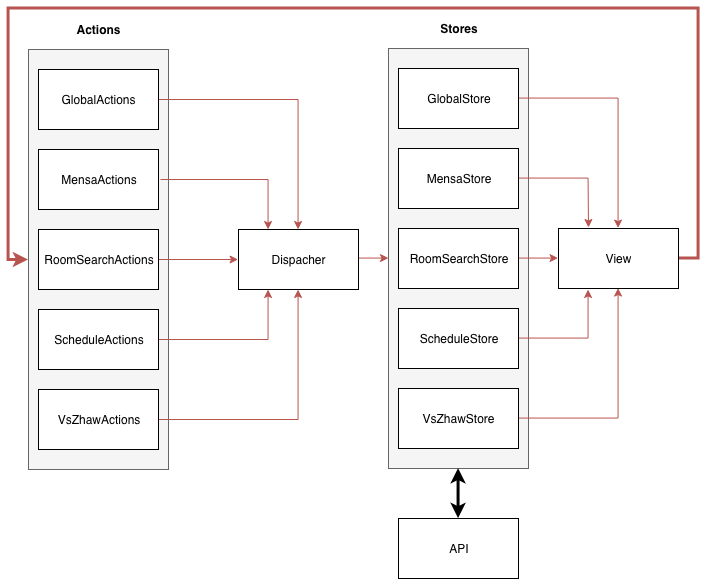
\includegraphics[width=14cm, center]{../../diagrams/flux.png}
  \captionsetup{width=13.5cm}
  \caption[Flux Pattern diagram]{\textbf{Flux Pattern diagram}: Unidirectional data flow from view React components through actions to the dispatcher singleton to stores. Views update based on changes in stores.}
  \label{fig:FluxDiag}
\end{figure}

\bigskip

### Service Worker

The data for the frontend is provided by the backend REST API. All data received from HTTP fetch requests is cached using a service worker \cite{ServiceWorker}. By caching the application data, we ensure that the user can still access all the information that was already loaded once. It also improves the loading speed of ZHAWo, since resources that have been cached are first served from cache, before the data is requested by the backend. After the fetch request has completed the cache is updated. With regard to, for example, a students schedule information, this practice makes a lot of sense since the actual data does not change often during the course of a semester.

In addition to offline caching, the service worker also allows users to install ZHAWo as a Progressive Web App (PWA) \cite{WhatIsPWA} to either their desktop or their mobile phone's home screen.

\newpage

## Test coverage

To test our application we used the framework Jest \cite{Jest} for both front- and backend. To test the React components, we used the GUI testing framework \cite{Enzyme} in addition to Jest.

For the express server application, we achieved a test coverage of 91\%. For the frontend React application 86\% of the code was covered, resulting in an overall project test coverage of about 87\% \cite{OurCoverage}. A detailed coverage can be found on our GitHub repository \cite{OurGithub} and on our Codecov page \cite{OurCoverage}.

Good testing practices and a high test coverage were important to us. Especially with our agile development approach, this was vital to maintan a high velocity by not introducing unexpected breaking changes between sprints.

## Metrics

Google provides the automated tool Lighthouse \cite{Lighthouse} to audit and rate PWAs. Besides providing performance metrics, Lighthouse can also be used to test various PWA aspects, including if the application still responds without network connection. ZHAWo achieved a performance rating of 100 out of 100, confirming the user feedback that the app has a very good performance (see Feedback Section \ref{feedback}). ZHAWo also passed all automated PWA checks confirming that it performs well even on slow networks and caching of offline content through the service worker works as intended. Manual tests confirm that as long as a resource such as a timetable or a mensa menu was previously fetched, the application still functions even without any connection to the internet. A detailed report of the Lighthouse audit can be found on the Github Repository \cite{OurGithub}.

During the last three weeks we published the application to a broader range of students, outside our small testing and feedback group. To date ZHAWo has had about 70 unique users. We were also positively surprised to see that the users were using the application for everything. To date the schedule has been used 411 times, the room search 295 times, the mensa 373 times and vszhaw 186 times. This user base consists of the participants of the survey and people who either heard about the application through those participants. It also consists of our testing group users. We expect the number of individual users to increase at the start of the next semester when we will send out an email about ZHAWo in collaboration with the vszhaw.

\begin{figure}[H]
  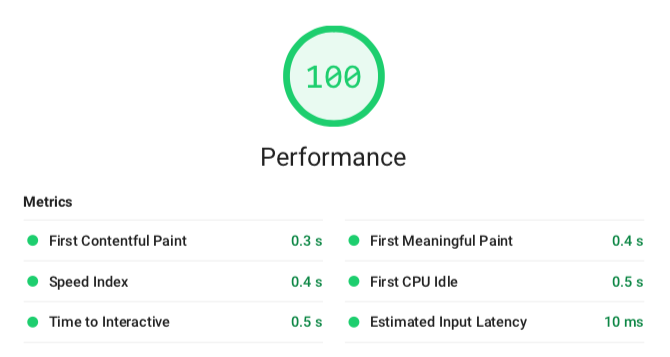
\includegraphics[width=10cm, center]{../../metrics/ZHAWoLighthousereportBAPreformance.png}
  \captionsetup{width=15.5cm}
  \caption [Lighthouse peformance audit]{\textbf{Lighthouse performance audit}: ZHAWo was rated by Lighthouse with a performance score of 100 out of 100 points.}
  \label{fig:LighthousePreformance}
\end{figure}

\newpage

\end{markdown}


